\documentclass{article}
\usepackage[utf8]{inputenc}

\title{Chem-131C-Lec5}

\author{swflynn }
\date{April 2017}

\usepackage{natbib}
\usepackage{graphicx}
\usepackage{braket}
\usepackage{amsmath}
\usepackage[margin=0.7in]{geometry}
\usepackage{subfigure}

\begin{document}

\maketitle

\section*{Lecture 5; 4/12/17}
Last Class we briefly mentioned Stirling's approximation as a method for evaluating the natural log of a factorial. 
The approximation is valid for big systems (as N gets very large).
\begin{equation}
    \ln N! \approx N \ln N - N + \cdots
\end{equation}
Here there are other terms that most people do not consider for first order approximations. 

\subsection*{The Gamma Function}
Consider the gamma function $\Gamma(z)$, if this is a new function to you... greetings! 
This function is the most common way to define the factorial in mathematics, and subsequently shows up alot in statistical mechanics and quantum mechanics.
\begin{equation}
    \Gamma(z) \equiv \int_0^\infty x^{z-1}e^{-x}dx
\end{equation}

Introduced by Legendre (famous guy, something known as Legendre transforms are how you derive all the thermodynamic potentials i.e.  Gibbs Free Energy, Helmholtz Free Energy etc).
It turns out that the definitions of the thermodynamics potentials are just Legendre transforms of the internal energy (if you take a graduate class on thermodynamics this will be the first few weeks of the course). 

If you consider the gamma function of (n+1) you can prove that this integral is actually equal to the factorial (n!). 
\begin{equation}
    \Gamma(n+1) = \int_0^\infty x^{n}e^{-x}dx = n!
\end{equation}
To solve this we notice that the exponential will not change in power, but we can reduce the power of the x term. 
This general format suggests to do integration by parts (IBP), so let: 
\begin{center}
  \begin{tabular}{ | l | c | }
    \hline
    u = x$^n$ & v = -e$^{-x}$ \\ \hline
    du = nx$^{n-1}$ dx & dv = e$^{-x}$dx  \\
    \hline
  \end{tabular}
\end{center}
Using our IBP substitutions we can evaluate this integral (note the uv terms both go to 0 when you evaluate them at the limits).
\begin{equation}
\begin{split}
    \int_0^\infty x^{n}e^{-x}dx &= x^n(-e^{-x}) \Big|_0^\infty - \int_0^\infty -e^{-x}nx^{n-1}dx \\
    &= n\int_0^\infty x^{n-1}e^{-x}dx
    \end{split}
\end{equation}
And here we start to see something interesting, let's repeat the IBP one more time to better see the pattern.
\begin{center}
  \begin{tabular}{ | l | c | }
    \hline
    u = x$^{n-1}$ & v = -e$^{-x}$ \\ \hline
    du = n-1x$^{n-2}$ dx & dv = e$^{-x}$dx  \\
    \hline
  \end{tabular}
\end{center}
\begin{equation}
\begin{split}
n\int_0^\infty x^{n-1}e^{-x}dx &= n\left[ x^{n-1}(-e^{-x})\right]\Big|_0^\infty - n\int_0^\infty (n-1)x^{n-2}e^{-x}dx \\
n\int_0^\infty x^{n-1}e^{-x}dx &= n(n-1)\int_0^\infty x^{n-2}e^{-x}dx \\
\cdots \\
\int_0^\infty x^{n}e^{-x}dx &= n!
\end{split}
\end{equation}
We now see the pattern, if we keep repeating this process we will keep integrating our (n-i) factors all the way down to 1 which is exactly the definition of n!

\subsection*{Stirling's Approximation}
Consider the integrand (the terms inside the integral) of the gamma function ($x^{n}e^{-x}$). 
In general when you want to understand an integral you should start by looking at the integrand itself, to see how your function behaves. 
The product of these two function is dictated by the x$^n$ term at smaller x, and eventually the long term will win and force the function back to 0.
Intuition says we expect a sharp peak upward initially, then the exponential will turn on and force the function steeply down to 0.
This is depicted in the graph below, even for a small n=10 (which is very small, n in real systems is very large) and 0$<$x$<$1.3 we see the product of the two terms (red curve) start to shoot up. 
If I just plot the integrand as shown in the second panel, even for a small n=10 the function gets huge and collapses back to 0 rather quickly. 
As noted on the graph, i will name the top of the peak x* for the derivations below. 
\begin{figure}[h!]
\subfigure[Individual Functions]{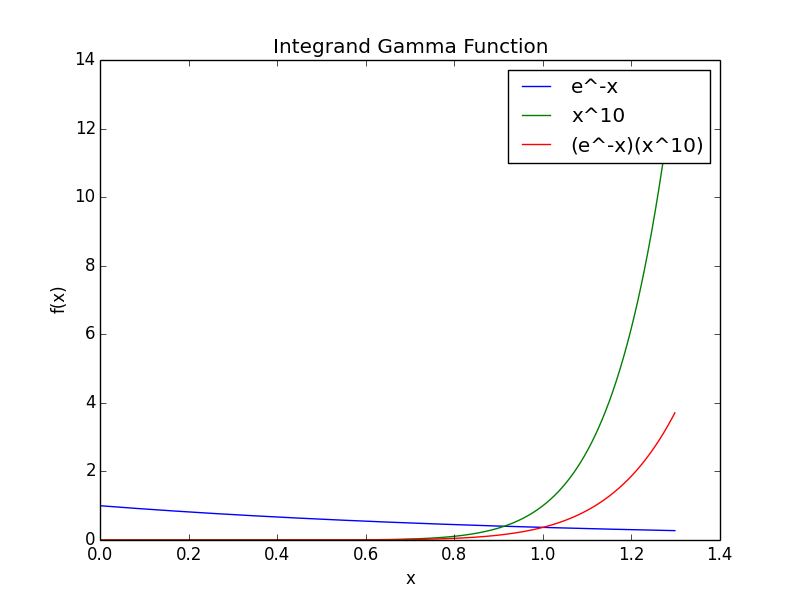
\includegraphics[scale=0.44]{scaling.png}}
\subfigure[Integrand Scaling]{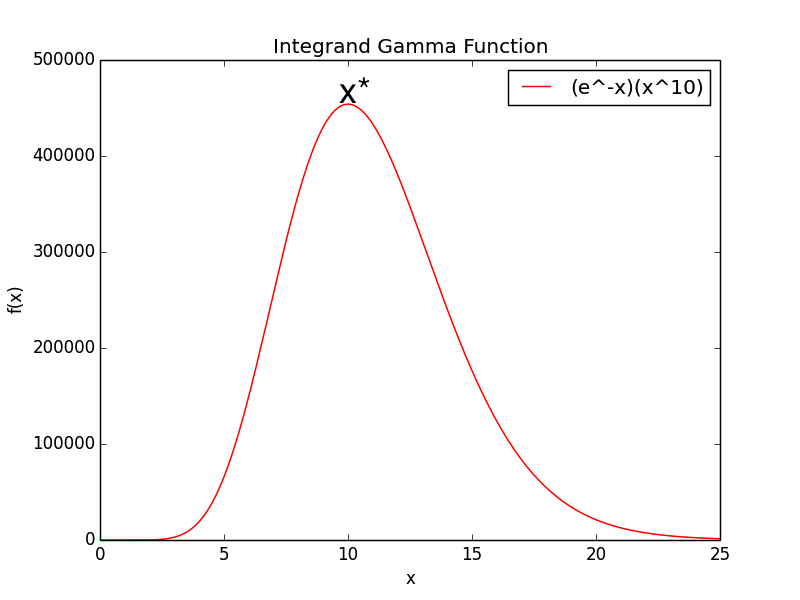
\includegraphics[scale=0.44]{integrand.png}}
\caption{Gamma Function Integrand Scaling}
\end{figure}
As you can imagine this function is not very well behaved and will take more mathematics than basic calculus to understand.

\subsubsection*{Asymptotic Approximation}
The question now is how do we integrate some function with a very steep peak (remember that is bad in calculus, is it actually a function?). 
Let's call x* the x value where our integrand reaches its sharp peak. 
We know as N gets larger this peak will get narrower and steeper, so maybe this limit will give us some insight into the functions integral. 
We can imagine the derivative of the function at x* must be 0, we are at the exact point where our function switches from growing to decaying and is therefore flat!
We are now going to use a \textbf{Taylor Series Approximation} to describe our function. 
So we will assume we can write our function of interest as the first few terms of a Taylor series expansion EXP$\left[ f(x*) + \frac{1}{2}f''(x*)(x-x*)^2 +\cdots \right ] \equiv e^{g(x)}$. 
So we are looking to solve for our Taylor Expansion function g(x) for our integral of interest (another way to say this we are assuming g(x) has the form of a Taylor expansion to the second order). 
The function we are interested in scales rapidly, to better grasp how this works we can write the function in terms of an exponential so that the scaling is not as drastic in this 'new space'.
\begin{equation}
\begin{split}
    \int_0^\infty x^{n}e^{-x}dx &= \int_0^\infty e^{\ln(x^n)-x}dx \\
    &= \int_0^\infty e^{n\ln(x)-x}dx
    \end{split}
\end{equation}
So we have now found our function of interest. 
We know that the first derivative evaluated at x* is 0 by construction, so we can use this. 
\begin{equation}
\begin{split}
g(x) &= n\ln(x) -x\\
\frac{dg}{dx} &= \frac{n}{x}-1 = 0 \implies x* = n \\
\frac{d^2g}{dx^2} &= \frac{-n}{x^2}  \\
\frac{d^2g(x*)}{dx^2} &= \frac{-n}{x*^2} = \frac{-n}{n^2} = \frac{-1}{n}
\end{split}
\end{equation}
So the overall approximation (second order Taylor Expansion of our function) is
\begin{equation}
\begin{split}
\int_0^\infty e^{n\ln(x)-x}dx &\approx  \int_0^\infty e^{f(x*) + 1/2f''(x*)(x-x*)^2} \\
&= \int_0^\infty e^{nln(n)-1 - (1/2n)(x-n)^2}dx \\
&= e^{n(\ln(n) -1)} \int_{-\infty}^\infty e^{(1/2n)(x-n)^2}dx \\
&= n\ln(n)-n(\sqrt{2\pi n})
\end{split}
\end{equation}
This completes our second order Taylor expansion about the peak of our function (x*). 
This new integral is an approximation, but is easy to solve, the first term is a constant, and the second order term is a Gaussian. 
I have switched the bounds (to make it a Gaussian), but our function is just some sharp peak, therefore the area under the curve from 0$\rightarrow -\infty$ is just 0. 

So the first order approximation to ln N! =  n ln(n) - n.
A second order approximation to the factorial function adds on the quadratic term ([-1/2n(x-n)$^2$] giving ln n! = nln(n)-n($\sqrt{2\pi n}$).
Of course you could keep adding terms from the Taylor expansion to make a better approximation. 

\subsection*{Thermodynamics....Finally!}
Moving on to thermodynamics: we are now studying macroscopic systems of interest and their surroundings.
We characterize systems using certain variables, such as the Temperature (T), and the internal energy (U). 
An \textbf{open} system allows for matter to be exchanged between the system and surroundings (usually what engineers study, chemists usually consider closed systems). 
A \textbf{diathermal} system allows heat transfer (q), an \textbf{adiabatic} system will not allow heat transfer (the system is well insulated or the process is done so fast heat cannot transfer).
Note q is the variable used to specify heat transfer.
Tn the context of thermodynamics there is no partition function (thermodynamics came first) do not confuse the two. 
In general, if the surroundings of your system are the universe, when the two reach equilibrium you can approximate the change in Temperature of the universe to be 0 (it is just too big). 
An \textbf{isolated system} has no heat or energy exchange. 
The \textbf{First Law of Thermodynamics} can be stated as $\Delta$U = 0 for isolated systems, also commonly stated as the conservation of energy. 
\begin{equation}
\begin{split}
    \Delta U &= q+w\\
    du &= \delta q+\delta w
\end{split}
\end{equation}
This is the most common form of the first law of thermodynamics, here q refers to the transfer of heat (you can't have 10 heat, it is a transfer of energy). 
The w is work, there are in general many different types of work such as electrochemical, mechanical, electromagnetic, etc.
Chemists are usually interested in PV work, the work done when a gas expands against the containers of a wall. 

\subsection*{State Functions}
Consider some function f(x,y), we can write the total differential of this function as follows. 
\begin{equation}
df = \frac{\partial f}{\partial x}dx + \frac{\partial f}{\partial y}dy
\end{equation}
For our purposes I like to think of a function that has a total differential as a function that has interchangeable partial derivatives. 
This may not seem intuitive, however, if you do graduate thermodynamics you will derive all the equations of thermodynamics, and this property \textbf{symmetry of second derivatives} is very important. $\frac{\partial^2f}{\partial x \partial y} = \frac{\partial^2f}{\partial y \partial x}$ This property is not always true!

I suggest this because things like work and heat do not have total differentials, you cannot write these functions in this way. 
We will explore this concept more, however, work and heat are path-dependent functions, meaning how you do them matters.
This should make sense, consider bringing your dishes to the sink, if you decide to dig a hole out of your room to the kitchen you probably did more work, then if you simply used the door, but hey the dishes got to the sink in both situations. 
We note this path dependence with the different change symbol when we are working with these types of functions. 

The potential energy is a state function, this means it has the total differential, and it does not matter how you got to a certain state, your energy is what it is. 
Intuitively, consider your potential energy at the top of a building, if you took the elevator, or the stairs doesn't matter, if you jump it will hurt the same. 
But you may be more tired from the stairs because you personally did more work!

\subsection*{On The System}
The first law can be written with either a plus or a minus between the heat and work. 
This is ultimately a matter of who you talk to, engineers use a minus because they want to know what work is available to be done by the system, what useful work is there. 
Chemists measure systems after perturbing them, so they want to do things on the system to see how they respond.
I personally suggest that you think about the problem physically and add the correct sign at the end of the problem. 

Although work can be very complicated, chemists (and especially and undergraduate course) will be most interested in mechanical work. 
From basic physics we know that. 
\begin{equation}
dw - -F_{ext}dx
\end{equation}
Here the force is an external force. 
We could imagine using a spring as our system, we could then assume it is an ideal spring that obeys Hooke's Law
\begin{equation}
F=-kx
\end{equation}
We will assume our system only has work, so we can calculate the potential energy. 
\begin{equation}
\Delta U = w = \int_0^x -Fdx = \int_0^x kdx = \frac{1}{2}kx^2
\end{equation}

As I stated above chemists are usually interested in PV work and ignore all other types of work for the first law. 
If you are working with an ideal gas then you know the EOS; PV=nRT. 
We also know the potential energy for an ideal gas (monoatomic) is $\frac{3}{2}$nRT. 
An important thing to note about this is that the U$\rightarrow$U(T) for an ideal gas (this is not true in general). 

\subsection*{Reversible Piston}
A final example for this lecture, consider the \textbf{reversible} compression of an ideal gas in a cylinder. 
We must do some work on the cylinder to move the piston in and compress the gas. 
What is the most efficient way to do this? 
Well what if we pushed on the cylinder just hard enough to overcome the pressure of the gas pushing back on the cylinder.
If we push infinitesimally harder than the pressure of the gas (and wait forever) we can move compress the gas. 
This hypothetical case is the reversible method, because we push so slow we can replace the external pressure with the pressure of the gas at every step of our process (we can only do this in the reversible case!). 
\begin{equation}
\begin{split}
   dw = -F_{ext}dx = \frac{F_{ext}}{A}Adx = -P_{ext}dx \\
   = -P_{gas,reversible}dV = \frac{nRT}{V}
\end{split}
\end{equation}
Remember this is only true if you push the cylinder reversibly!
 
\section{Supplemental Notes}
This lecture was a bit heavy mathematically, you would not be expected to do derive the Stirling's approximation on an undergraduate exam, however, you will be expected to use it!
Remember it is a good approximation as n gets large. 
\subsection*{Integration by Parts}
As you are aware the integral of a function is much harder to calculate than the derivative. 
Unfortunately we usually need the integral of a function if we want to calculate macroscopic quantities like temperature or energy.
Integration by parts is one method for calculating integrals, by replacing the integral of interest with a different one. 
The method itself comes directly from the product rule as we will show below. 
Consider some function a(x) that is a product of 2 other functions f and g.  
\begin{equation}
    a(x) = f(x)g(x)
\end{equation}
Let's take the derivative of a (I will denote a derivative as a prime to save typing).
\begin{equation}
    \frac{d}{dx}\left[f(x)g(x)\right] = f(x)g'(x) + g(x)f'(x)
\end{equation}
Now take the anti-derivative of both sides. 
\begin{equation}
    \begin{split}
        \int\frac{d}{dx}\left[f(x)g(x)\right] &= \int f(x)g'(x) + \int g(x)f'(x) \\
         \left[f(x)g(x)\right] &= \int f(x)g'(x) + \int g(x)f'(x) 
    \end{split}
\end{equation}
Now we can simply rearrange our equation to find a formula for our integral of interest. 
\begin{equation}
    \int f(x)g'(x) =  \left[f(x)g(x)\right] + \int g(x)f'(x) 
\end{equation}
This is our integration by parts formula, a direct result of the product rule of derivatives. 
It tells us that if we have a function to integrate where the integrand looks like a function multiplied by the derivative of another function we are in luck. 
Practically speaking if one term in the integrand can be integrated easily, and the other term can be differentiated easily you should give IBP a try. 

\subsection*{Taylor Series Approximation}
I will try to do a brief summary of approximating functions using Taylor Expansions. 
The main take-away is that we can approximate a function as a summation of higher and higher order polynomials. 
It turns out if you keep guessing high order polynomials you can keep getting a more accurate representation of a very complicated function you are interested in.
For this to work your complicated function of interest must be defined for all ($\forall$) x, and it's derivative must also be defined $\forall$ x (the function is somewhat well behaved).
So the method essentially replaced the complicated function of interest with a summation of higher order polynomials and their derivatives evaluated at a certain point.
The most common time you see this approach is in physics, where we find a point of interest such as the peak of a sharp function.
It is very common to take that peak and do a Taylor expansion about that point as an approximation for the more complicated function itself. 

The method works like this, consider our function of interest (the complicated one) as f(x) and we want to replace it with a polynomial p(x). 
Let's call our point of interest a. 
So our first guess would be....well at a we better have our function and polynomial be equal.
\begin{equation}
    p(x) \approx f(a)
\end{equation}
Graphically this is just a horizontal line that will touch f(a). 
As you can guess this is not a good approximation of our function, but it is a start. 
Where do we go from here, well let's start taking derivatives!
The next approximation will require our polynomial to have the same first derivative as our function when we evaluate them at a. 
\begin{equation}
    p(x) \approx f(a) + f'(a)x
\end{equation}
This says make our polynomial equal to the function at a and make it have the same derivative (remember the first derivative is the slope, the tangent line). 
So now we don't just have a horizontal line, we have a tangent line at the point a!
Hopefully the pattern is becoming clear, we can keep demanding higher order derivatives to be equal to our function at point a, and we will get a better and better guess. 
So our third guess for what this polynomial could be would require the second derivative to be the same as well. 
\begin{equation}
    p(x) \approx f(a) + f'(a)x + \frac{1}{2}f''(a)(x-a)^2
\end{equation}
Note the (x-a) is just because we are not considering our function at 0, we are looking at some point a and we need to shift the entire function over. 
The 1/2 factor comes from the derivative, if you take a second derivative you will get a factor of 2, so we just normalize it with 1/2. 
Higher derivatives will get different factors to normalize. 
The general formula for the Taylor series (this approximation is the Taylor series, the Maclaurin series sets a=0) is 
\begin{equation}
  P(x) \approx \sum_{i=1}^n f^i(a) \frac{(x-a)^i}{i!}
\end{equation}
So the big picture, we have a function that is too complicated. 
Maybe I can just approximate that function as a sum of polynomials. 
If I want the integral of that complicated function, maybe I can assume most of the area under the curve occurs at the highest point of the function a. 
So let's just evaluate all of our polynomials at a and add them up. 

\end{document}
